% Inbuilt themes in beamer
\documentclass{beamer}

% Theme choice:
\usetheme{Dresden}
\usecolortheme{whale}

% packages
%\usepackage[hmargin=2cm, vmargin=2cm]{geometry}
\usepackage{microtype}
\usepackage{adjustbox}
\usepackage{graphicx}
\usepackage{hyperref}
\usepackage[english]{babel}
\usepackage{setspace}
%\usepackage{xcolor}
\usepackage{multicol}
\usepackage{float}
\usepackage{amsmath}
\usepackage{amssymb}
\usepackage[font=small,skip=2pt]{caption}
\captionsetup[figure]{labelformat=empty}
\usepackage[
backend=biber,
style=authoryear-comp,
]{biblatex}

\addbibresource{../RMbibliography.bib}
\parindent=0pt

 \newcommand{\independent}{\perp\!\!\!\!\perp} 

% Title page details: 
\title{Scalar on Function Regression \\
with Applications to Near-Infrared Spectroscopy}
\author{Jonathan Willnow, Jakob Juergens, Jonghun Baek}
\date{18.01.2022}

\begin{document}
	
	% Title page frame
	\begin{frame}
		\titlepage 
		\begin{center}
			{\small
			Research Module in Econometrics and Statistics \\
			Winter Semester 2021/2022}
		\end{center}
	\end{frame}
	
	% Remove logo from the next slides
	\logo{}
	
	% I'm not really a fan of a table of contents in short presentations (Jakob)
	% Outline frame
	%\begin{frame}{Outline}
	%	\tableofcontents
	%\end{frame}
	
	\begin{frame}{Introduction}
	
		\begin{itemize}
			\item \textbf{Near-Infrared} (NIR) \textbf{Spectroscopy} enables fast diagnostics by using the NIR region of the electromagnetic spectrum (from 780 nm to 2500 nm)
			\item Suited for field-monitoring / on-line analysis
			\item Spectroscopy results in high-dimensional dataset.	
			\item This set of measurements serves as set of discretized approximations of smooth spectral curves
			\item Regression to determine relationship between octane rating and spectral curves
			\end{itemize}
	\end{frame}
	
	\begin{frame}{Theory}
		A simple functional dataset is given by 
		$$\{x_{i}(t_{j,i}) \in \mathbb{R} \: \vert \: i = 1,2,...,N, \; j = 1,2,..., J_i, \; t_{j,i} \in [T_1, T_2] \}$$
		
		\begin{itemize}
			\item Continuous underlying process, where $x_i(t)$ exists $\forall t \in [T_1, T_2]$
			\item Only observed at $x_{i}(t_{j,i})$
			\item Example: Gasoline dataset (60 x 400)
			\item Other Examples: Growth curves, financial data, human perception (pitch), ...
			
		\end{itemize}
	\end{frame}

	\begin{frame}{Random Function}
		A \textbf{Random Variable} is a function $X : \Omega \rightarrow \mathcal{S}$ which is defined on a common probability space $(\Omega, \mathcal{F}, \mathbb{P})$ where $\Omega$ is a probability space with a $\sigma$-algebra $\mathcal{F}$ and a probability measure $\mathbb{{P}}.$
		\vspace{0.2cm}
		
		\begin{itemize}
			\item If $\mathcal{S} = \mathbb{R}$ then $X$ is a random variable
			\item If $\mathcal{S} = \mathbb{R}^{n}$ then $X$ is a random vector
			\item If $\mathcal{S}$ is a space of functions, $X$ is called a \textbf{Random Function}
		\end{itemize}
	\end{frame}

	\begin{frame}{Random Function}
		Let $\mathbb{E}$ be the index set and this can be described as
		$${X = \{X(t,\omega) : t \in \mathbb{E}, \omega \in \Omega\},}$$
		where $X(t, \cdot)$ is $\mathcal{F}$-measurable function on the sample space $\Omega$.\\
		\begin{itemize}
			\item It can be shortened to $X(t)$ by omitting $\omega$
			\item The function is realized when the $X(t)$ exists $\forall t \in \mathbb{E}$
		\end{itemize}
	\end{frame}

	\begin{frame}{Plots}
		\begin{minipage}{.5\textwidth}
			\begin{figure}
				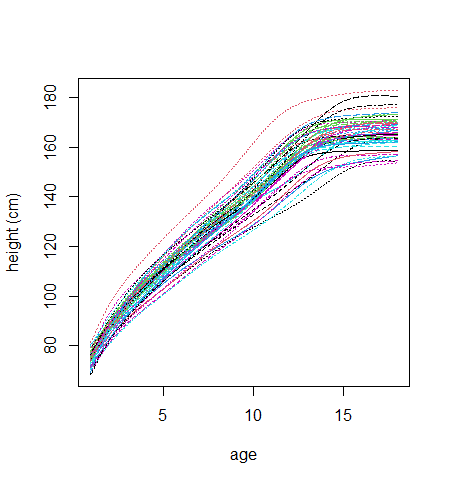
\includegraphics[width=\textwidth]{../Graphics/Growth_curves.png}
				\caption{Growth curves of \\ 54 girls age 1-18}
			\end{figure}
		\end{minipage}%
		\begin{minipage}{.5\textwidth}
			\begin{figure}
				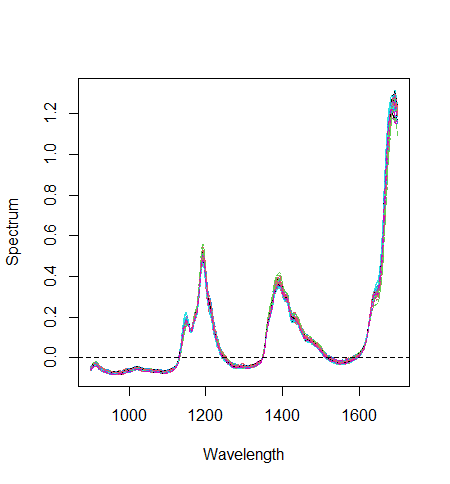
\includegraphics[width=\textwidth]{../Graphics/NIR.png}
				\caption{NIR spectrum of 60 \\ gasoline samples}
			\end{figure}
		\end{minipage}
	\end{frame}
	
	\begin{frame}{Square Integrable Function}
		If a function $f(t)$ satisfies
		$$\int_{0}^{1} \left(f(t)\right)^{2}dt < \infty$$
		the function $f(t)$ is called \textbf{Square Integrable Function} written $f(t) \in \mathbb{L}^{2}[0,1]$.
		\begin{itemize}
			\item Without loss of generality, the interval is defined in $[0,1]$.
			\item $\mathbb{L}^{2}$ is the set of all square integrable functions.
		\end{itemize}
	\end{frame}
	
	\begin{frame}{Square Integrable Function}
		Let $f, g \in \mathbb{L}^{2}[0,1]$, then we can define inner product by
		%$$(ab + bg)(t) = af(t) + bg(t), \quad t \in [0,1] and \forall a,b$$
		%, where $a$ and $b$ are scalars. (Maybe don't need)\\
		%We can additionally define the inner product as follows:
		$$\langle f,g \rangle = \int_{0}^{1} f(t)g(t)dt$$
		%\begin{itemize}
		%	\item
		\begin{itemize}
			\item Orthogonality of two different functions with $\langle f,g \rangle = 0$
			\item Distance between functions
		\end{itemize}
	\end{frame}
	
	%\begin{frame}{Stochastic Process Perspective}
	%	Functional data are the sample curves observed from continuous time stochastic precess.\\
	%	\begin{itemize}
	%		\item From this perspective, $X(t)$ is a random variable (?)\\
	%		\item $X(\cdot)$ is a collection of random variables by each time index(?)\\
	%		\item Realizations of a random function belong in large collection of functions
	%	\end{itemize}		
	%\end{frame}
	

	\begin{frame}{Basis Expansion}
		\textbf{Basis Expansion} is a linear combination of functions as described:
		
		$$X_{i}(t) = \sum_{k=1}^{\infty} c_{ik}\phi_{k}(t) \approx \sum_{k=1}^{K} c_{ik}\phi_{k}(t), \quad i = 1, \dots, n, \quad \forall t \in \mathbb{E}$$
		
		where $\phi_{k}(t)$ is the $k^{th}$ basis function of the expansion and $c_{ik}$ is the corresponding coefficient. We truncate the basis at $K$ to:
		\vspace{0.2cm}
		
		\begin{itemize}
			\item make the function smoother
			\item replace the original curves $X_{i}(t)$ by a smaller collection of $c_{nm}$
			%\item replace the original scalar data $X_{n}(t_{jn})$ by a smaller collection of $c_{nm}$
		\end{itemize}		
	\end{frame}
	
	%\begin{frame}{Two Typical Types of Basis Function}
	%	\textbf{Fourier Basis Function} is an element of the set:
	%	
	%	$$\{\sqrt{2}sin(2\pi nx | n \in \mathbb{N})\} \cup \{\sqrt{2}cos(2\pi nx | n \in \mathbb{N})\} \cup \{1\}$$
	%	
	%	%$$f(x) = a_{0} + \sum_{n=1}^{\infty}a_{n}cos(2\pi nx) + b_{n}sin(2\pi nx)$$	\\
	%	
	%	\vspace{2\baselineskip}
	%	\textbf{B-spline Basis Function} is a polynomial function defined by order and knots. \\
		
	%\end{frame}
	
	\begin{frame}{Basis Functions}
		\textbf{Fourier Basis Functions} are elements of the set:
		$$\{\sqrt{2}\sin(2\pi nx) | n \in \mathbb{N}\} \cup \{\sqrt{2}\cos(2\pi nx) | n \in \mathbb{N}\} \cup \{1\}$$
		\vspace{-0.5cm}
		\begin{figure}
			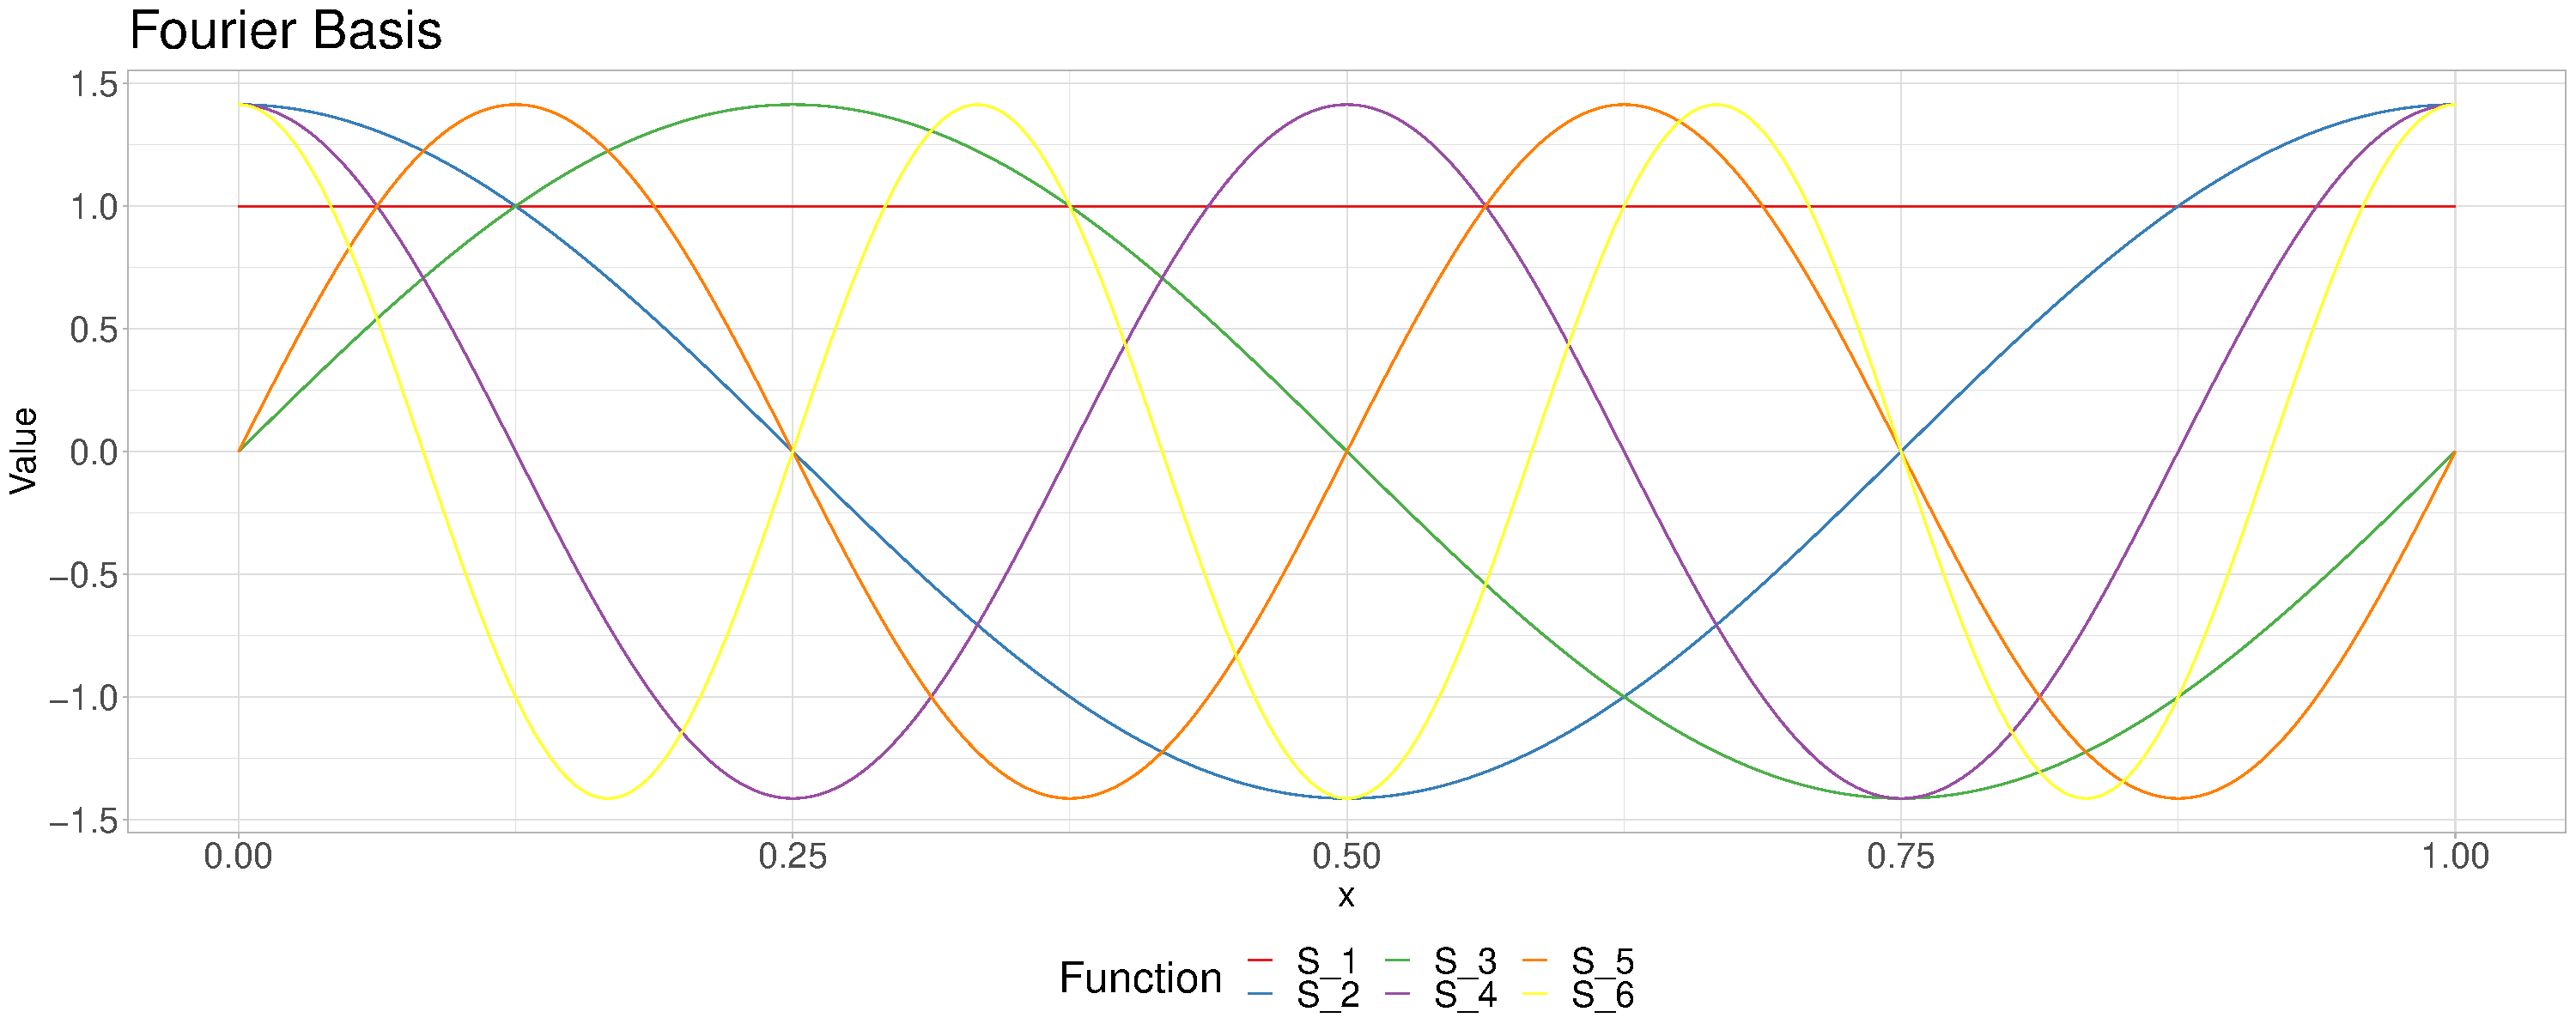
\includegraphics[width = \textwidth]{../Graphics/Fourier_Basis.pdf}
			%\caption {Fourier basis functions}
		\end{figure}
			
	\end{frame}
	
	\begin{frame}{Basis Functions}
		\textbf{B-spline Basis Functions} are polynomial functions defined by an order and a set of knots.
		\begin{figure}
			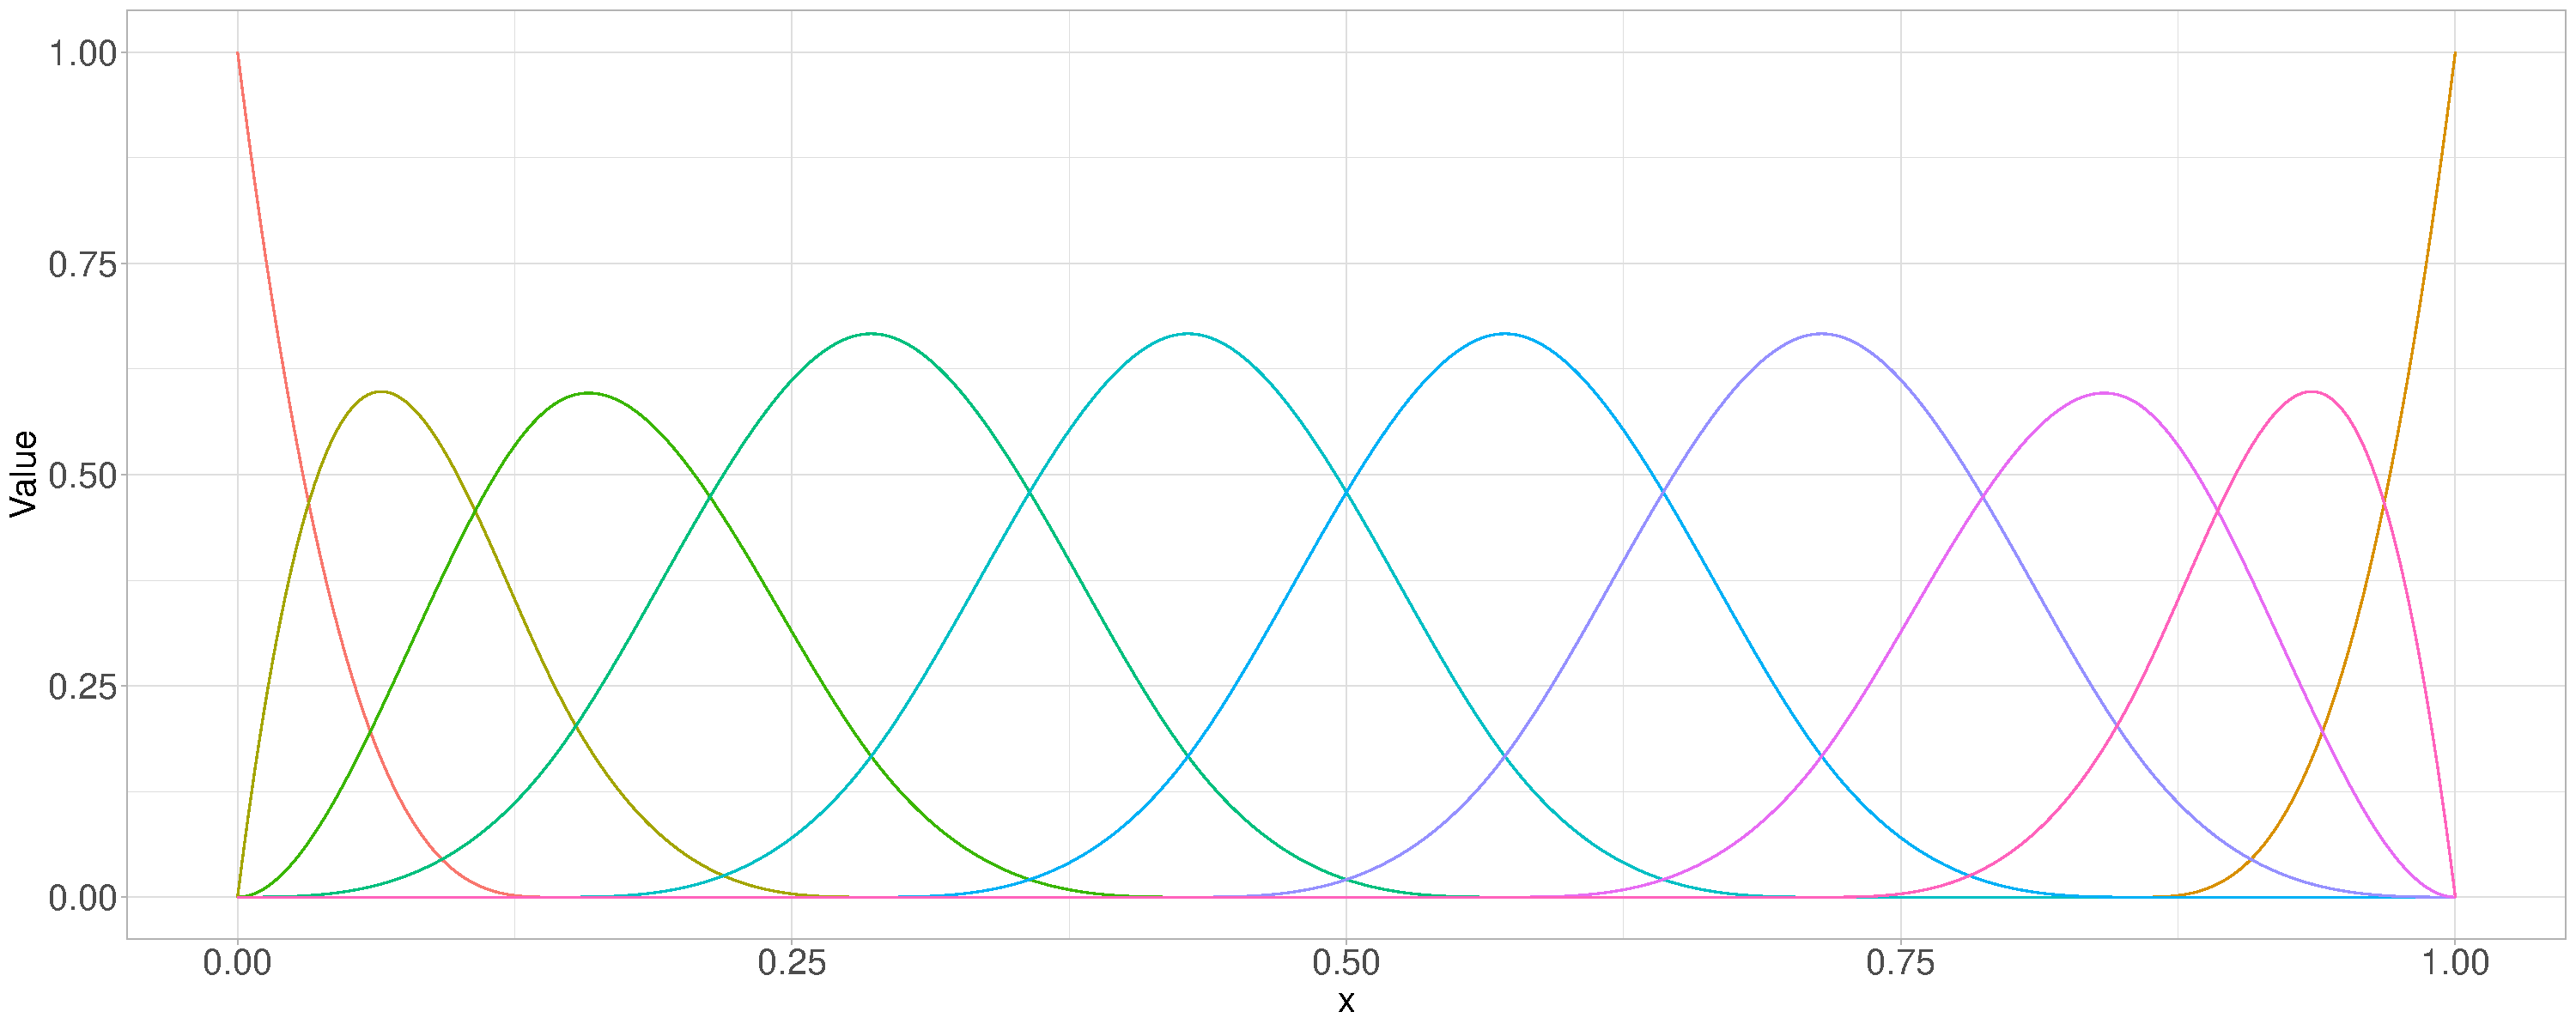
\includegraphics[width = \textwidth]{../Graphics/Bspline_Basis.pdf}
			%\caption {Bspline basis functions}
		\end{figure}
	\end{frame}
	
	\begin{frame}{Trade Off between Bias and Variance}
		How do we choose the number $K$ of basis functions?
		
		$$\textbf{MSE}[\hat{X}(t)] = \textbf{Bias}^2[\hat{X}(t)] + \textbf{Var}[\hat{X}(t)]$$
		
		$$\textbf{MISE}[\hat{X}] = \int_{0}^{1} \textbf{MSE}[\hat{X}(t)] dt$$
		
		\begin{itemize}
			\item The larger $K$, the better fit to the data, but also more fitting noise
			\item If $K$ is too small, the expansion would miss some significant information
		\end{itemize}
	\end{frame}
	
	\begin{frame}{Trade Off between Bias and Variance}
		\begin{figure}\notag
			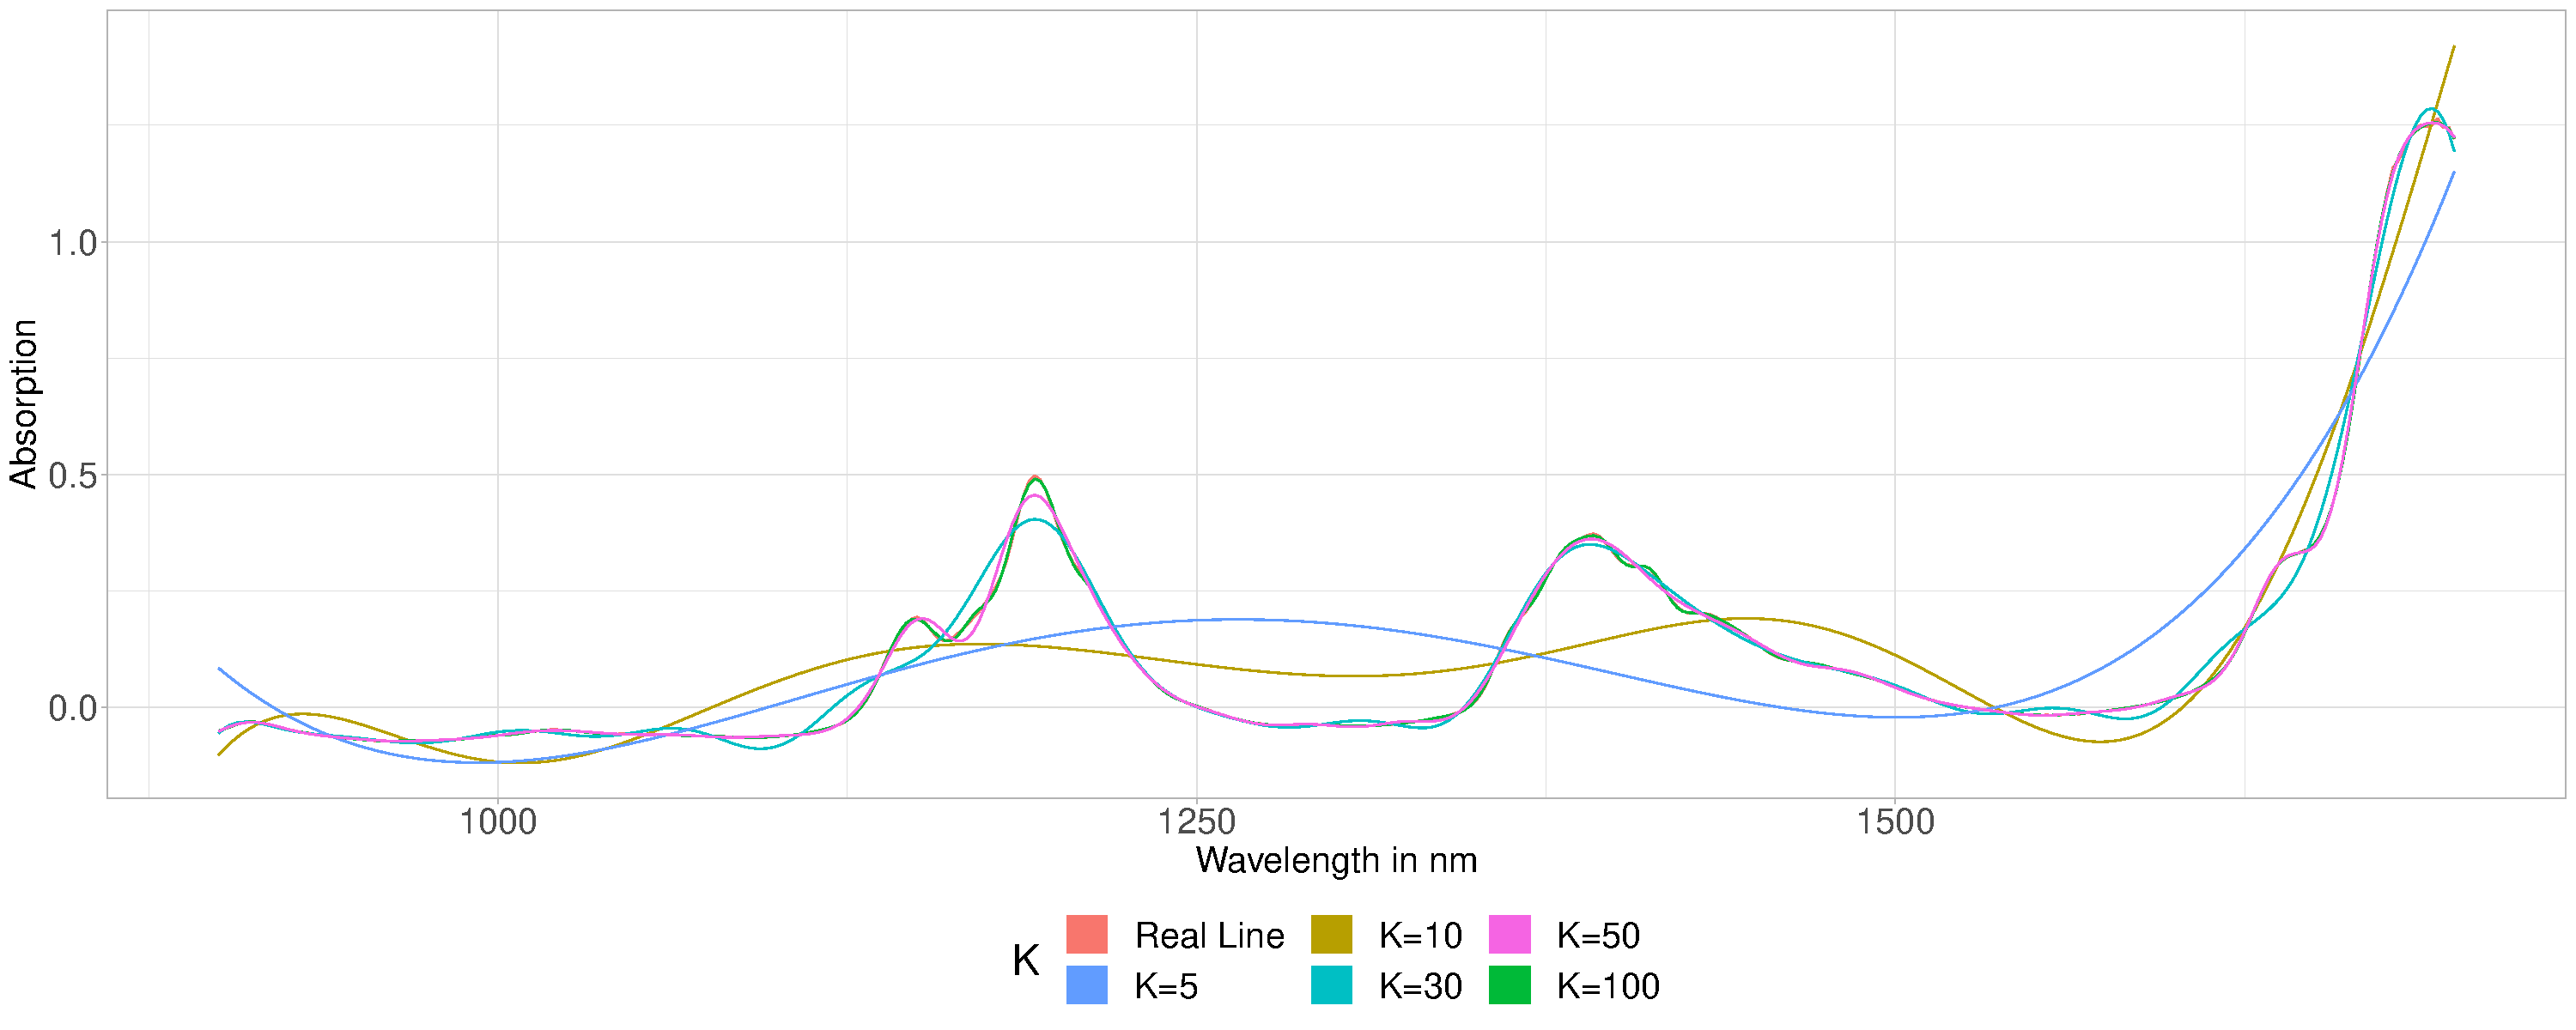
\includegraphics[width = \textwidth]{../Graphics/basis_expansions.pdf}
		\end{figure}
	\end{frame}

	\begin{frame}{Estimation via Basis Representation}
		Assume the following \textbf{Data Generating Process}
		$$Y(\omega) = \alpha + \int_{0}^{1} \beta(s) X(\omega)(s) \mathrm{d}s + \epsilon(\omega)$$
		\vspace{-0.6cm}
		\begin{itemize}
			\item $Y(\omega)$ and $\epsilon(\omega)$ realize in $\mathbb{R}$ and $X(\omega)$ realizes in $\mathbb{L}^2[0,1]$
		\end{itemize}
		\vspace{0.3cm}
					
		Let $\{\phi_i(t) \: \vert \: i = 1, \dots, \infty\}$ be a basis of $\mathbb{L}^2[0,1]$ leading to the following representation of $\beta(t)$
		
		$$\beta(t) = \sum_{j = 1}^{\infty} c_j \phi_j(t) \approx \sum_{j = 1}^{L} c_j \phi_j(t)$$
		%Assume that we have a data set containing observations each of which is made up of:
		%\begin{itemize}
		%	\item $y_i$: a scalar realization of $Y(\omega)$ - the octane rating of gasoline
		%	\item $x_i(t)$: a realization of $X(\omega)$ - the measured NIR spectrum
		%\end{itemize}

	\end{frame}

	\begin{frame}{Estimation via Basis Representation}
		We can transform the data generating process into:
		\begin{equation}\notag
			\begin{split}
				Y(\omega) & = \alpha + \int_{0}^{1}\left[\left(\sum_{j = 1}^{\infty} c_j  \phi_j(s)\right) X(\omega)(s) \right]\mathrm{d}s + \epsilon(\omega) \\
						  & = \alpha + \sum_{j = 1}^{\infty} \left[c_j \textcolor{red}{\int_{0}^{1} X(\omega)(s) \phi_j(s)\mathrm{d}s}\right] + \epsilon(\omega)	 \\
						  & = \alpha + \sum_{j = 1}^{\infty} c_j {\color{red}Z_j(\omega)} + \epsilon(\omega)  \approx  \alpha + \sum_{j = 1}^{L} c_j {\color{red}Z_j(\omega)}  + \epsilon(\omega)
			\end{split}
		\end{equation}
	
		Where a $Z_j(\omega)$ is a \textbf{scalar random variable}.
	\end{frame}

	\begin{frame}{Estimation via Basis Representation}
		Truncating the functional basis allows us to estimate coefficients using \textbf{multivariate regression} leading to an estimated coefficient vector $\hat{c} \in \mathbb{R}^L$ and an approximated coefficient function $\hat{\beta}(t)$:
		\vspace{-0.2cm}
		$$\hat{\beta}_L(t) = \sum_{j = 1}^{L} \hat{c}_{L,j} \phi_j(t)$$
		
		This is dependent on...\vspace{-0.2cm}
		\begin{multicols}{2}
			\begin{itemize}
				\item The basis $(\phi_j(t))_{j \in \mathcal{I}}$ for the estimation of $\beta(t)$
				\item The truncation parameter $L$\vfill\null
				\item The basis $(\psi_j(t))_{j \in \mathcal{I}}$ used for the observations
				\item The truncation parameter for the observations $K$
			\end{itemize}
		\end{multicols}

	\end{frame}

	\begin{frame}{Karhunen-Lo\'{e}ve Expansion}
		
		\textbf{Mean Function}: $$\mu(t) = \mathbb{E}\left[ X(\omega)(t) \right]$$

		\textbf{Autocovariance Function}: $$c(t,s) = \mathbb{E}\big[ \left( X(\omega)(t) - \mu(t) \right) \left( X(\omega)(s) - \mu(s) \right) \big]$$
		
		The \textbf{Eigenvalues} and \textbf{Eigenfunctions}: $\{(\lambda_i, \nu_i) \: \vert \: i \in \mathcal{I}\}$  are solutions of the following equation:
		$$ \int_{0}^{1}c(t,s)\nu(s) \mathrm{d}s = \lambda \nu(t) $$
	\end{frame}
	
	\begin{frame}{Karhunen-Lo\'{e}ve Expansion}\label{KLE}
		A random function $X(\omega)$ can be expressed in terms of its mean function and its Eigenfunctions:
		$$X(\omega)(t) = \mu(t) + \sum_{j = 1}^{\infty} \xi_j(\omega) \nu_j(t)$$
		
		Where the $\xi_j$ are scalar-valued random variables with the following properties.
		\begin{multicols}{2}
			\begin{enumerate}
				\item $\mathbb{E}[\xi_i(\omega)] = 0$
				\item $Var(\xi_i(\omega)) = \lambda_i$
				\item $Cov(\xi_i(\omega), \xi_j(\omega)) = 0$ for $i \neq j$
			\end{enumerate}
		\end{multicols}
		
		This is called the \textbf{Karhunen-Lo\'{e}ve Expansion} of $X(\omega)$ and the Eigenfunctions can serve as a basis. \\
		
		\hyperlink{spectral}{\beamergotobutton{Spectral Representation of Random Vectors}}
	\end{frame}

	\begin{frame}{Functional Principal Component Analysis}
		\textbf{Principal Component Analysis} can be extended to functional regressors in the form of \textbf{Functional Principal Component Analysis} (FPCA).
		\vspace{0.4cm}
		
		\textbf{Empirical Mean Function}:
		$$\hat{\mu}(t) = \frac{1}{n}\sum_{j = 1}^{n}x_j(t)$$

		\textbf{Empirical Autocovariance Function}:
		$$\hat{c}(t,s) = \frac{1}{n} \sum_{j = 1}^{n} \left(x_j(t) - \hat{\mu}(t)\right) \left(x_j(s) - \hat{\mu}(s)\right)$$

	\end{frame}

	\begin{frame}{Functional Principal Component Analysis}\label{FPCA}
	
		The \textbf{Eigenvalues} and \textbf{Eigenfunctions}: $\{(\hat{\lambda}_i, \hat{\nu}_i) \: \vert \: i \in \mathcal{I}\}$  are solutions of the following equation:
		$$ \int_{0}^{1}\hat{c}(t,s)\hat{\nu}(s) \mathrm{d}s = \hat{\lambda} \hat{\nu}(t) $$
		\vspace{0.2cm}
		
		The $\{\hat{\nu}_i(s) \: \vert \: i \in \mathcal{I}\}$ are called \textbf{Functional Principal Components} and can serve as a basis for representing the original curves. 
		\vspace{0.2cm}
		
		The corresponding scores $\hat{\xi}_i$ can be derived as
		$$\hat{\xi}_j(\omega) = \int_{0}^{1} (F(\omega)(s) - \hat{\mu}(s)) \hat{\nu}_j(s) \mathrm{d}s$$
		
		\hyperlink{PCA}{\beamergotobutton{PCA for Random Vectors}}
	\end{frame}

	\begin{frame}{FPCA - Plot}
			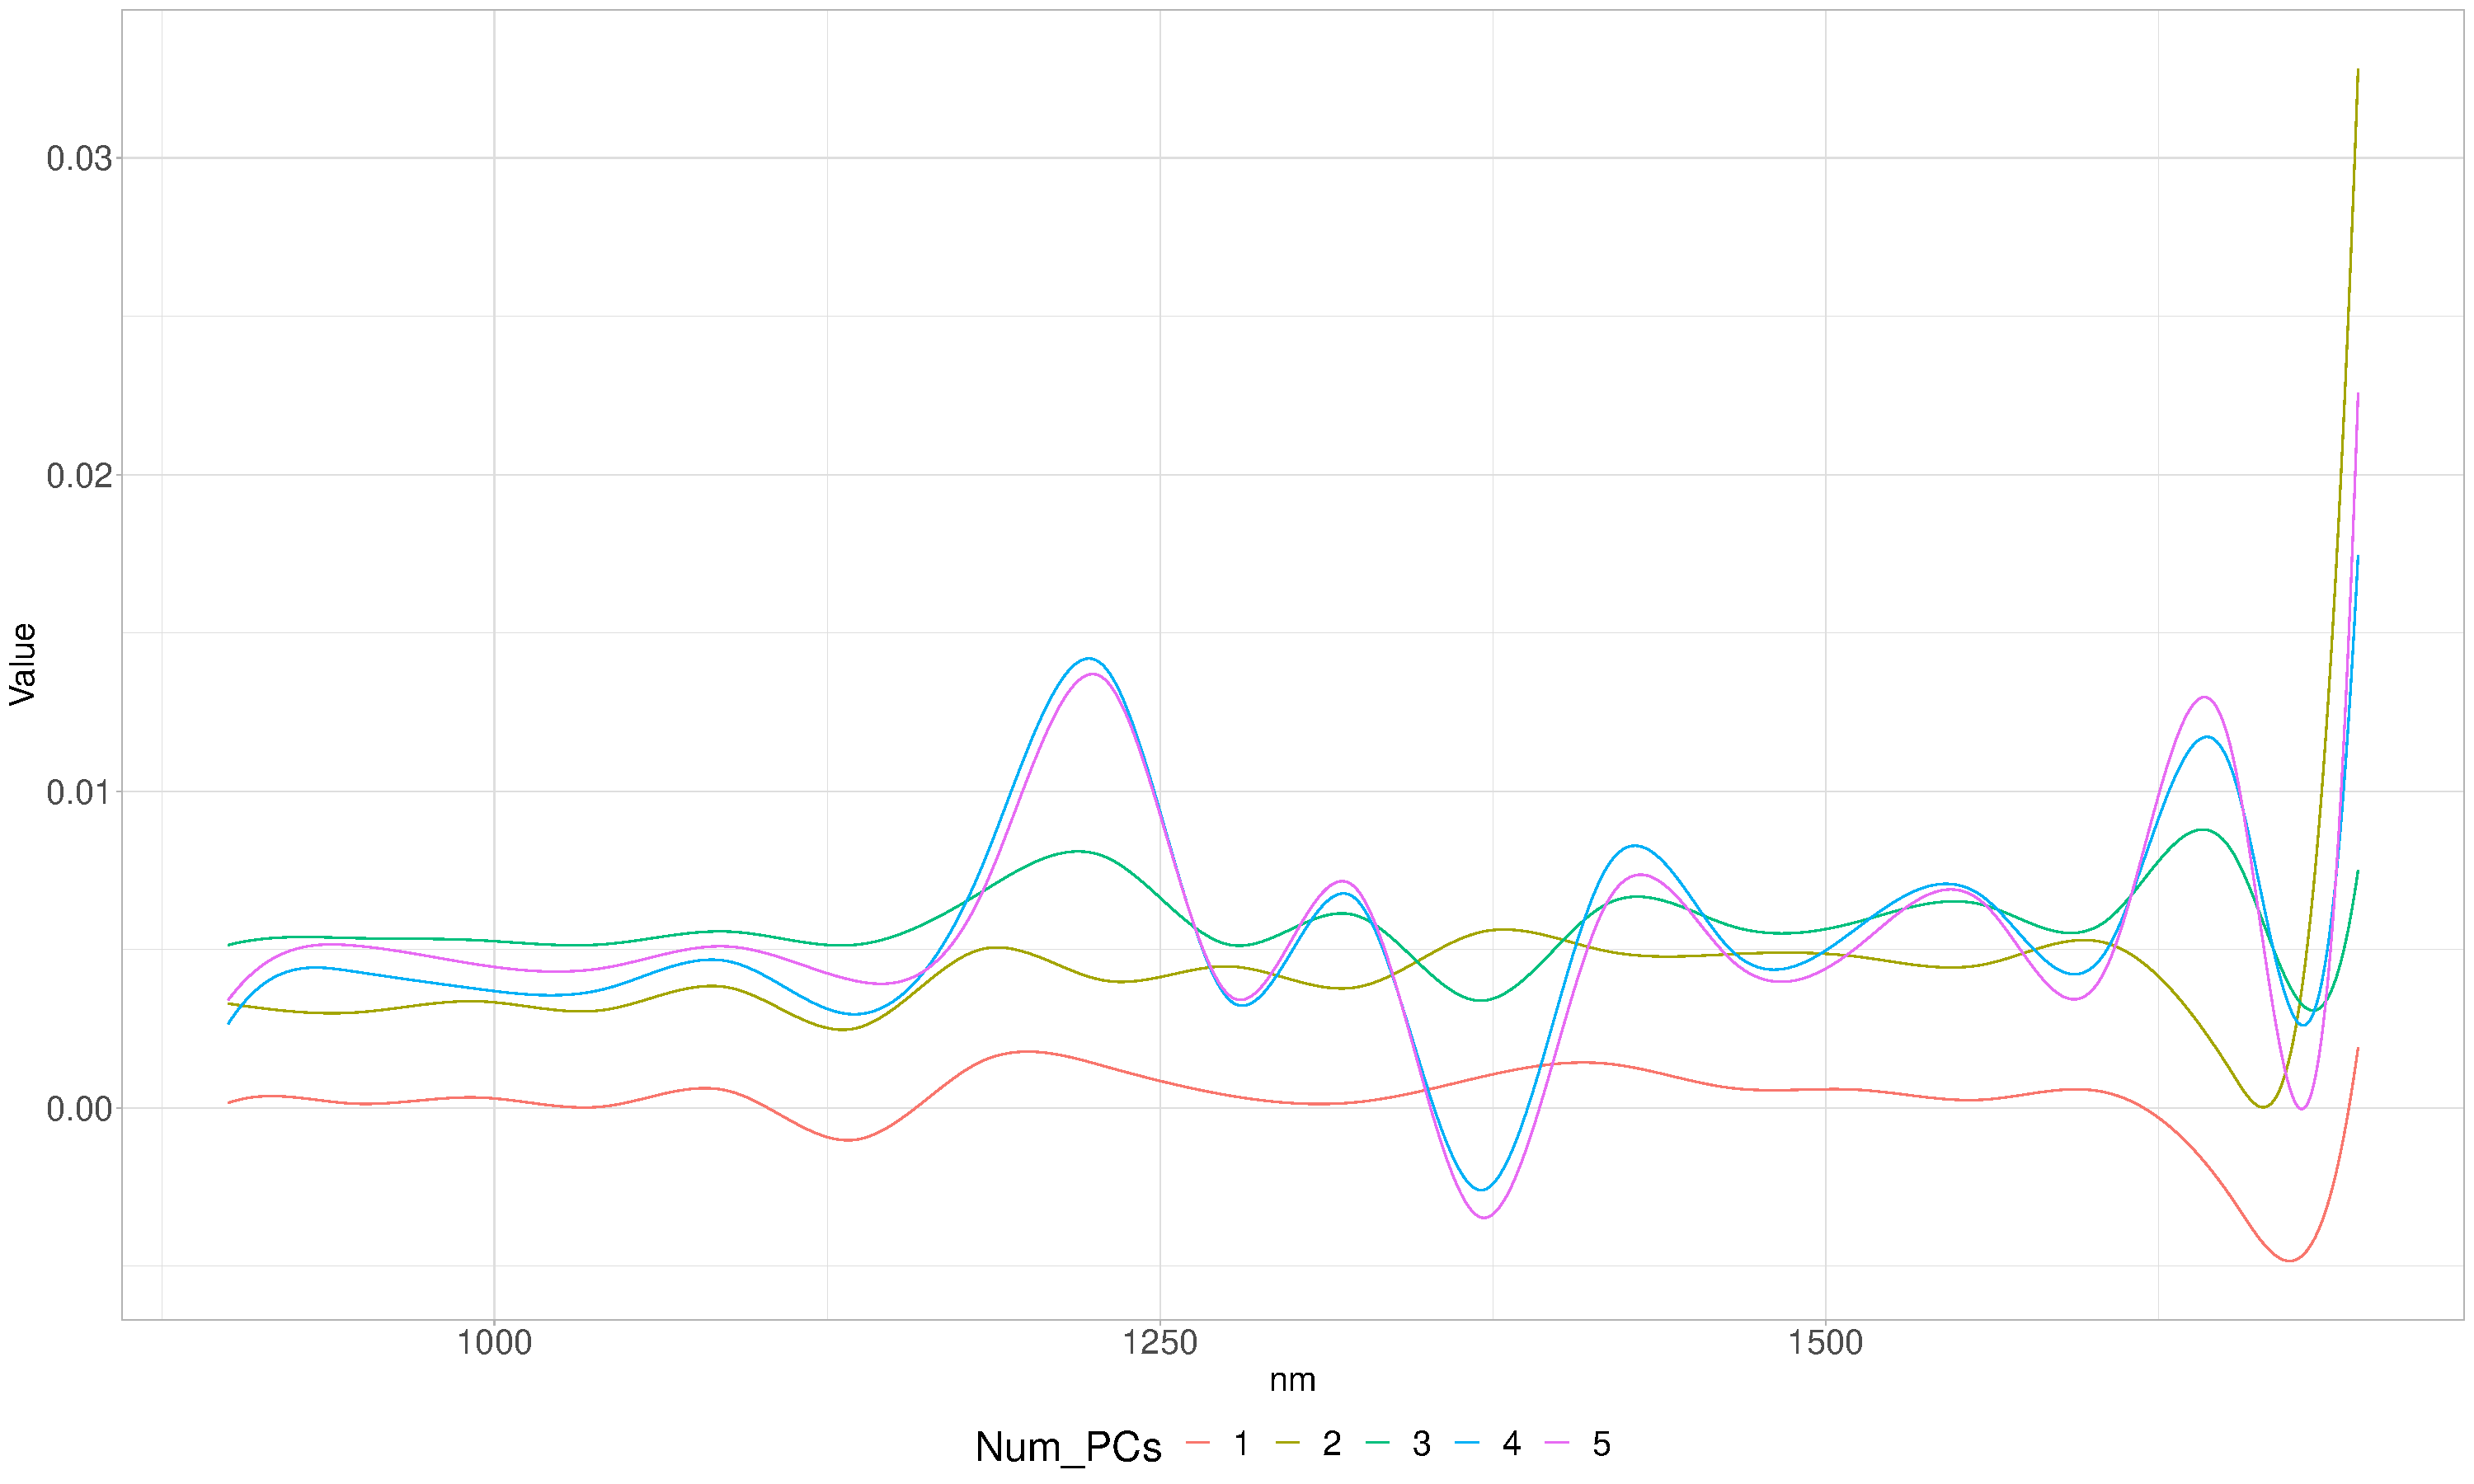
\includegraphics[width = \textwidth]{../Graphics/pc_approx.pdf}
	\end{frame}
	

	\begin{frame}{Simulation Setup}
		\begin{itemize}
			\item Use the \textbf{Gasoline Dataset} (NIR-spectroscopy, 60 $\times$ 401) to predict octane ratings.
			\item Generate \textbf{similar curves} from gasoline dataset:
		\end{itemize}
	
		$$\tilde{X}(\omega)(t) = \hat{\mu}(t) + \sum_{j = 1}^{J} \tilde{\xi}_j(\omega) \hat{\nu}_j(t)$$ 

		\begin{itemize}
			\item $\tilde{\xi}_{j} \sim \mathcal{N}(0,\hat{\lambda}_j)$ and $\tilde{\xi}_{j} \independent \tilde{\xi}_{k}$ for $j \neq k$
			\item Simplification: the $\xi_{j}$ do not follow a normal
			\item $\tilde{X}(\omega)(t)$, $\hat{\mu}(t)$ and $\hat{\nu}_j(t)$ are approximated as vectors in $\mathbb{R}^{401}$.
		\end{itemize}
		
	\end{frame}
	
	
	\begin{frame}{Simulation Setup cont.}

		Following \textbf{Reiss and Ogden (2007)}, let $f_1(t)$ and $f_2(t)$ be two coefficient functions: 

		\vspace{0.1cm}
		\begin{figure}
			\centering
			\begin{minipage}{.5\textwidth}
				\centering
  				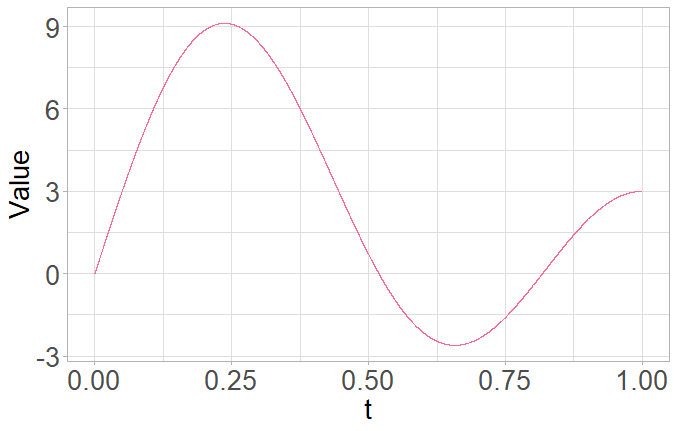
\includegraphics[width=\textwidth]{smooth_function.png}
  				\caption{$f_1(t)$, smooth function}
  				\label{fig:test1}
			\end{minipage}%
			\begin{minipage}{.5\textwidth}
	  			\centering
  				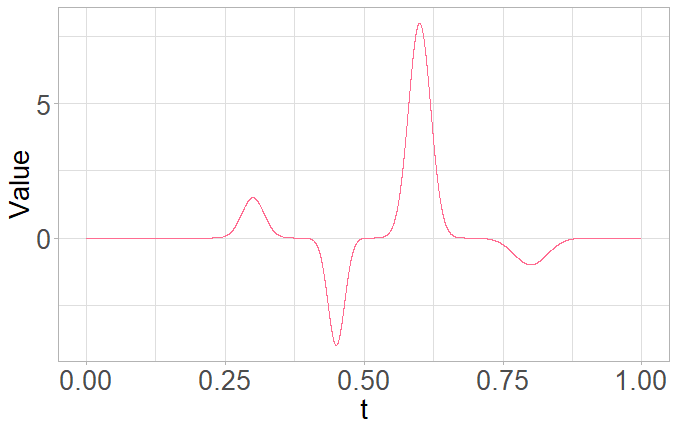
\includegraphics[width=\textwidth]{bumpy_function.png}
  				\caption{$f_2(t)$, bumpy function}
  				\label{fig:test2}
			\end{minipage}
		\end{figure}
		
	\end{frame}	

	
	\begin{frame}{Simulation Setup cont.}
		Let 
		$$Y_{1,f} = \langle NIR, f\rangle + Z\left(  \frac{var(\langle NIR, f\rangle)}{0.9} - var(\langle NIR, f\rangle)\right)$$ 
		$$Y_{2,f} = \langle NIR, f\rangle + Z\left( \frac{var(\langle NIR, f\rangle)}{0.6} - var(\langle NIR, f\rangle)\right)$$
		
		where $Z \sim \mathcal{N}(0,1)$ be two responses for $f \in \{f_1(t), f_2(t)\}$.	
		\begin{itemize}
    		\item Four combinations with different number of cubic basis-function $n_{basis} \in (4,5,...,25)$ and fourier functions $(1,3,...,25)$ to perform regression using basis expansion and the FPCR approach.
			\item Compare results via criteria (CV, Mallows CP,...)
		
		\end{itemize}
	\end{frame}
	
	
	\begin{frame}{Recap: Trade Off between Bias and Variance}
		\begin{figure}\notag
			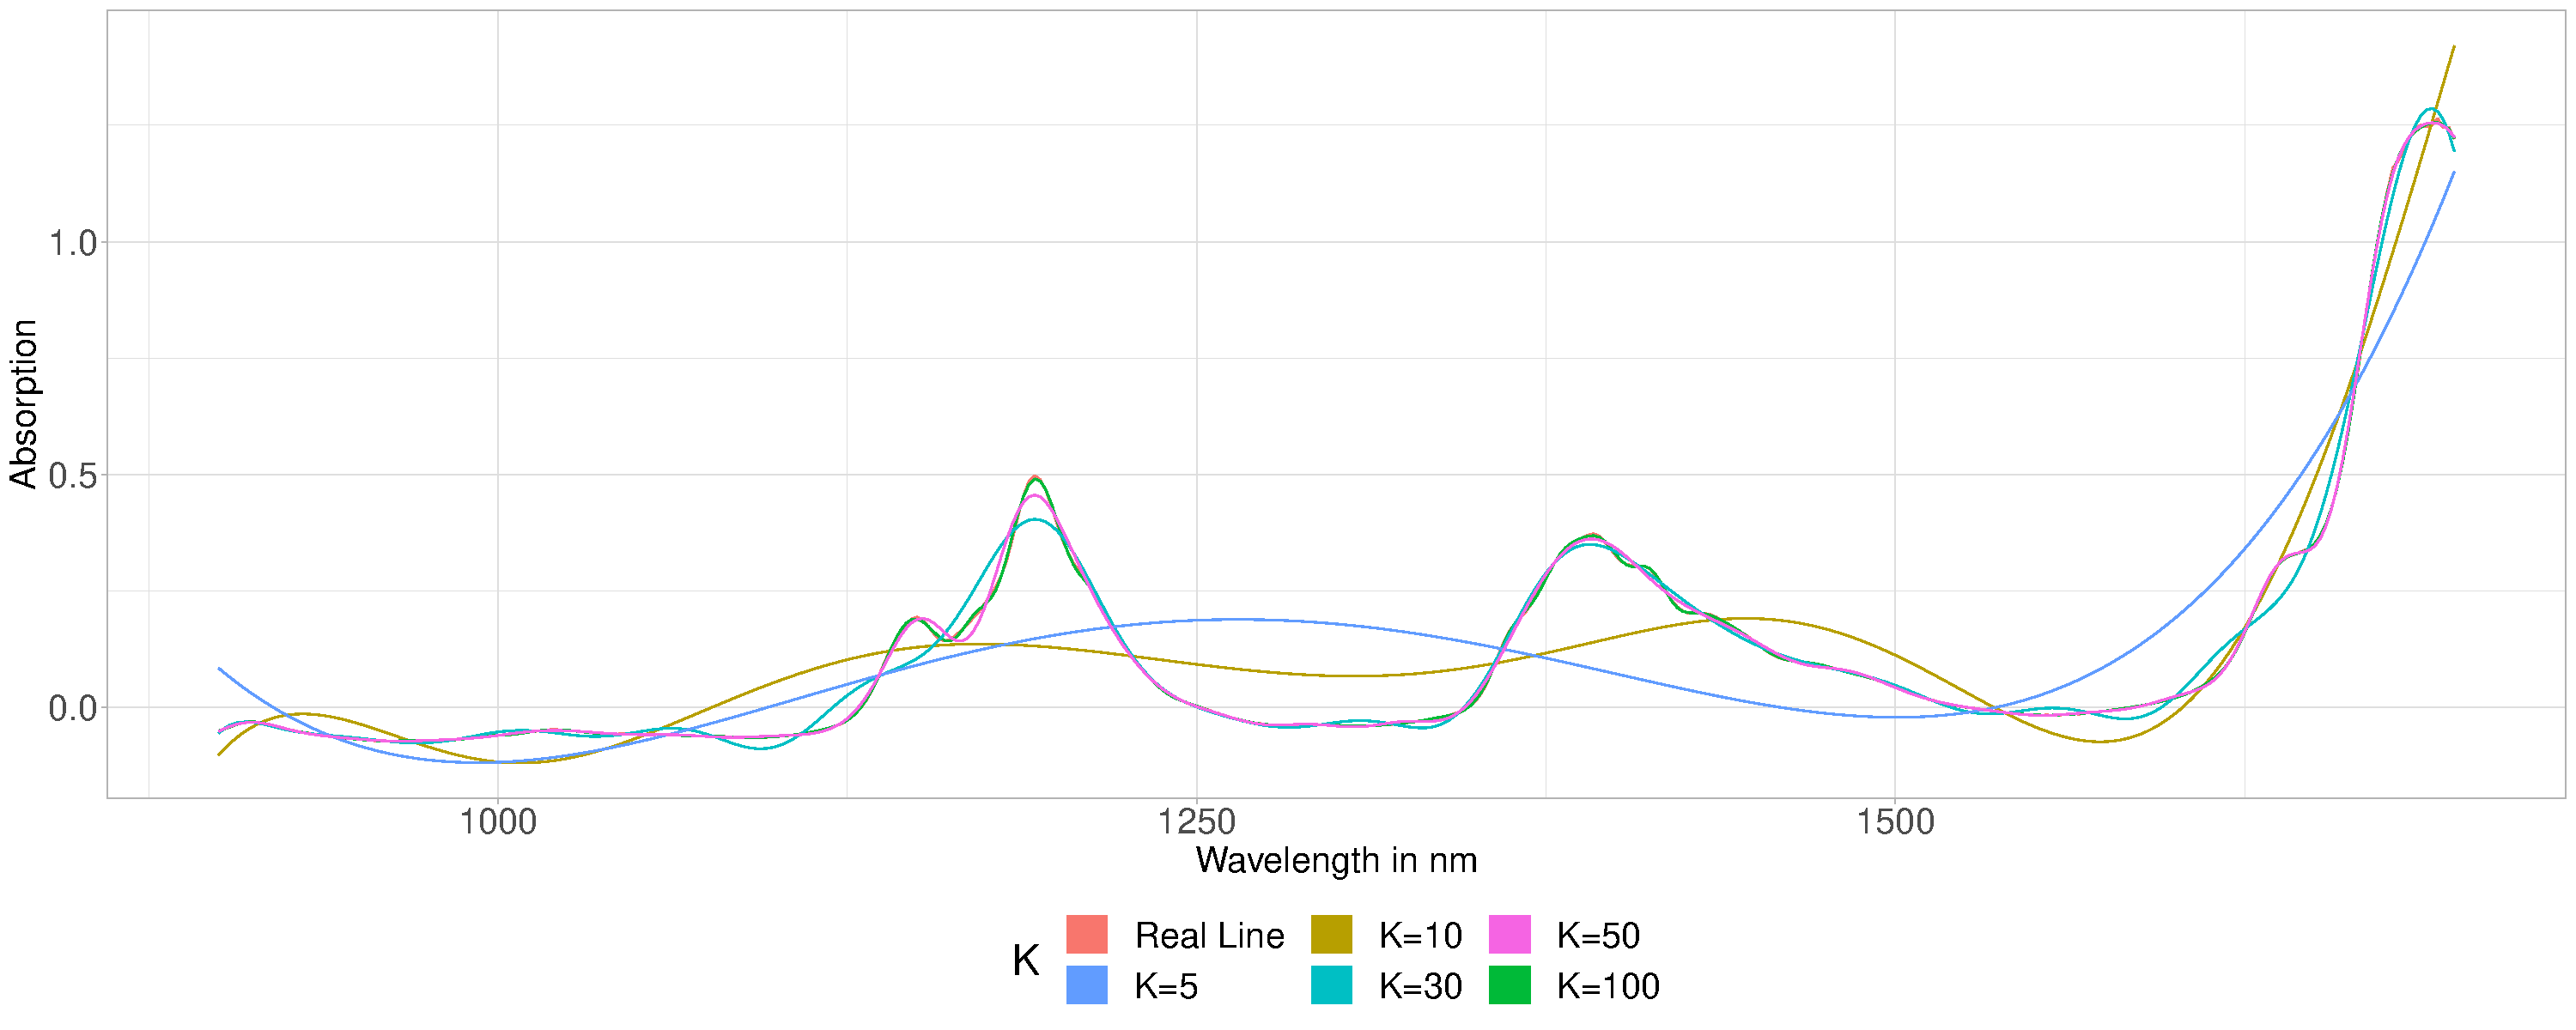
\includegraphics[width = \textwidth]{../Graphics/basis_expansions.pdf}
		\end{figure}
	\end{frame}
	
	
	
	
	\begin{frame}{Simulation Results - bspline}
		\begin{table}
		\centering
\resizebox*{\columnwidth}{6.5cm}{%
\begin{tabular}{lllllll}
\cline{2-6}
 & \textbf{f1\_e1\_spline}                 & \textbf{f1\_e2\_spline}                 & \textbf{f2\_e1\_spline}                   & \textbf{f2\_e2\_spline}                 & \textbf{n\_basis} &  \\ \cline{2-6}
 & 2.13178119016857                        & {\color[HTML]{FD6864} 71.7099603226115} & 0.608171495504618                         & 1.53453412563582                        & 4                 &  \\
 & 2.00756061672648                        & 71.9395214288329                        & 0.342736147598609                         & 1.29059813220677                        & 5                 &  \\
 & {\color[HTML]{FD6864} 1.99374215191544} & 72.2563479644725                        & 0.245623228181924                         & 1.20138156565603                        & 6                 &  \\
 & 2.03648199621352                        & 73.7857088138923                        & 0.279709073157873                         & 1.24948462939122                        & 7                 &  \\
 & 2.18614795862507                        & 79.0485254545422                        & 0.104397806306425                         & 1.145842683177                          & 8                 &  \\
 & 2.05113790304629                        & 74.1783834857012                        & 0.0355899940503619                        & {\color[HTML]{FD6864} 1.02172959116332} & 9                 &  \\
 & 2.10522981230773                        & 76.1883552769234                        & 0.029691294210754                         & 1.03929073546751                        & 10                &  \\
 & 2.1011969989178                         & 76.4030798206724                        & {\color[HTML]{FD6864} 0.0296057602994908} & 1.04246508005367                        & 11                &  \\
 & 2.38150697658292                        & 86.1706579685565                        & 0.0369986801764011                        & 1.18191116948046                        & 12                &  \\
 & 2.21136870222925                        & 80.6207607207599                        & 0.0363026864816967                        & 1.10242516644568                        & 13                &  \\
 & 2.44947712911835                        & 87.6976578759761                        & 0.0380185616636571                        & 1.21257716080672                        & 14                &  \\
 & 2.28870905624113                        & 83.4755186453129                        & 0.0315198808793299                        & 1.13630733462095                        & 15                &  \\
 & 2.5490614406393                         & 93.593040512565                         & 0.0351718970102256                        & 1.26520057279256                        & 16                &  \\
 & 2.55139454545527                        & 93.3074090320499                        & 0.0352440364348144                        & 1.26610962599564                        & 17                &  \\
 & 2.75160520792553                        & 100.556190093422                        & 0.0380316879790874                        & 1.3620304183365                         & 18                &  \\
 & 3.02429148497643                        & 109.987580398216                        & 0.0409879625688711                        & 1.4813467852555                         & 19                &  \\
 & 3.42548075922108                        & 122.395980857659                        & 0.0471595536208038                        & 1.68537882583396                        & 20                &  \\
 & 3.63355571510069                        & 132.077208928751                        & 0.0490939239286374                        & 1.7750377827367                         & 21                &  \\
 & 5.93680459997264                        & 209.128064205703                        & 0.0779161032701813                        & 2.86105576687348                        & 22                &  \\
 & 9.63325470698287                        & 339.676032195418                        & 0.126422677097386                         & 4.65363116820157                        & 23                &  \\
 & 15.2728939666428                        & 545.827184915647                        & 0.200212312881423                         & 7.22652606521015                        & 24                &  \\
 & 13.9781506322669                        & 495.957265678323                        & 0.184269309019229                         & 6.6968929082163                         & 25                & 
\end{tabular}%
}
\end{table}
	\end{frame}
	
	
	
	\begin{frame}{Simulation Results - Fourier}
		\begin{table}
		\centering
\resizebox*{\columnwidth}{!}{%
\begin{tabular}{lllllll}
\cline{2-6}
 & \textbf{f1\_e1\_spline}                 & \textbf{f1\_e2\_spline}                 & \textbf{f2\_e1\_spline}                   & \textbf{f2\_e2\_spline}                 & \textbf{n\_basis} &  \\ \cline{2-6}
 & 2.02918344408687                       & {\color[HTML]{FD6864} 72.0085477229407} & 0.511999648510189                         & 1.47468049635309                         & 3                &  \\
 & {\color[HTML]{FD6864} 2.0220366421201} & 72.60172284215                          & 0.16157756089415                          & 1.13746697354709                         & 5                &  \\
 & 2.0354924731897                        & 73.1836346250812                        & 0.0293072016650537                        & {\color[HTML]{FD6864} 0.990682620987463} & 7                &  \\
 & 2.06199840536677                       & 73.9631412481736                        & {\color[HTML]{FD6864} 0.0290190767234641} & 0.999385186246351                        & 9                &  \\
 & 2.08808310984254                       & 75.0920660376146                        & 0.0290873388349217                        & 1.01393568534507                         & 11               &  \\
 & 2.09974789215127                       & 75.9422236701681                        & 0.0294100223429063                        & 1.02909474969485                         & 13               &  \\
 & 2.1086767501285                        & 76.7123085769457                        & 0.0298036585996321                        & 1.03713735705978                         & 15               &  \\
 & 2.13013296583489                       & 77.4907530428231                        & 0.0300236821233963                        & 1.03980406503428                         & 17               &  \\
 & 2.15348157839283                       & 78.3942553410957                        & 0.030307463717998                         & 1.0508902800978                          & 19               &  \\
 & 2.17750745519215                       & 79.2057575714294                        & 0.0306501467540424                        & 1.06172373892826                         & 21               &  \\
 & 2.20581113466118                       & 80.3800790338639                        & 0.0309985992677207                        & 1.07695651700849                         & 23               &  \\
 & 2.23717951397715                       & 81.5089652049561                        & 0.0314869147262958                        & 1.09052842774153                         & 25               & 
\end{tabular}%
}
\end{table}
	\end{frame}
	
	
	
		
		
		
	\begin{frame}{Application setup}
		\begin{itemize}
		\item
    		Use insights from the simulation study to uncover dependence.
    		\item
    		Similar setup, but using only bspline basis expansion and initial 60 spectral curves.
    		\item
    		Validation set approach:	Scores of test data needs to be estimated by the training data. 
    		\item
    		Report results by MSE scaled by variance.
		\end{itemize}
	\end{frame}
	
	%\begin{frame}{Summary}
	%	\begin{itemize}
	%	\item
    %		Concepts of functional data: 
    %		\begin{itemize}
	%		\item See dataset as smooth curve than as set of discrete measurements.
    %			\item Theory of Random Functions, motivated from random variable.
    %			\item Basis expansion and its Bias-Variance tradeoff.
    %			\item Scalar on Function Regression via Basis Expansion.
    %			\item Functional principal component Analysis and FPCR.
	%	\end{itemize}
    %		\item
    %		Simulation study results: specification depends on function and signal-to-noise ratio
    %		\item
    		% Guided you  from the beginning to the end of the presentaion through one application ....
    %		Guided through application to predict octane ratings.
    		
	%	\end{itemize}
	%\end{frame}
	
	\begin{frame}{Further Reading}
		\nocite{hsing_theoretical_2015}
		\nocite{kokoszka_introduction_2017}
		\nocite{Bohacs_Ovadi_Salgo1998}
		\nocite{FR_li_et_al_2020} 
		\nocite{Reiss_2007b}
		\nocite{ramsay_functional_2005}
		\AtNextBibliography{\tiny}
		\printbibliography[heading=none]
	\end{frame}
	
	% From here on out are the supplementary slides.
	
	\begin{frame}{Spectral Representation of Random Vectors}\label{spectral}
		Let $X(\omega)$ be a random vector realizing in $\mathbb{R}^p$.
		
		\begin{itemize}
			\item Let $\mu_x = \mathbb{E}(X)$ and $\Sigma_X = Cov(X)$
			\item Let $\{\gamma_i \: \vert \: i = 1, \dots, p\}$ be the orthonormal \textbf{Eigenvectors} of $\Sigma_X$
			\item Let $\{\lambda_i \: \vert \: i = 1, \dots, p\}$ be the corresponding \textbf{Eigenvalues} of $\Sigma_X$
		\end{itemize}
		
		\vspace{0.2cm}
		Then $X$ can also be represented as
		$$X(\omega) = \mu_x + \sum_{i = 1}^{p} \xi_i(\omega) \gamma_i$$
		where the $\xi_i(\omega)$ have the following properties
		
		\begin{multicols}{2}
			\begin{enumerate}
				\item $\mathbb{E}[\xi_i(\omega)] = 0$
				\item $Var(\xi_i(\omega)) = \lambda_i$
				\item $Cov(\xi_i(\omega), \xi_j(\omega)) = 0$ for $i \neq j$
			\end{enumerate}
		\end{multicols}
	
		\hyperlink{KLE}{\beamergotobutton{Karhunen-Lo\'{e}ve Expansion}}
	\end{frame}

	\begin{frame}{Principal Component Analysis}\label{PCA}
		A related concept is \textbf{Principal Component Analysis} (PCA).
		\vspace{0.2cm}
		
		$\Sigma_X$ unknown $\rightarrow$ \textbf{sample analogues}
		
		\begin{itemize}
			\item Let $\mathbf{X} \in \mathbb{R}^{n \times p}$ contain the standardized regressors
			\item Let $\hat{\Sigma}_X = \frac{\mathbf{X}'\mathbf{X}}{n}$
			\item Let $\{\hat{\gamma}_i \: \vert \: i = 1, \dots, p\}$ be the orthonormal \textbf{Eigenvectors} of $\hat{\Sigma}_X$
			\item Let $\{\hat{\lambda}_i \: \vert \: i = 1, \dots, p\}$ be the corresponding \textbf{Eigenvalues} of $\hat{\Sigma}_X$
		\end{itemize}
		\vspace{0.2cm} 
		
		Then $Z_i(\omega) = \hat{\gamma}_i' X(\omega)$ is called the i'th principal component and
		\begin{multicols}{2}
			\begin{enumerate}
				\item $\mathbb{E}[Z_i(\omega)] = 0$
				\item $Var(Z_i(\omega)) = \hat{\lambda}_i$
				\item $Cov(Z_i(\omega), Z_j(\omega)) = 0$ for $i \neq j$
			\end{enumerate}
		\end{multicols}
		\hyperlink{FPCA}{\beamergotobutton{Functional Principal Component Analysis}}
	\end{frame}
\end{document}